\documentclass[12pt, a4paper]{ctexart}
\usepackage{amsmath, amsthm, amssymb, appendix, bm, graphicx, hyperref, mathrsfs}
\usepackage{indentfirst} % 用于开头空两格
\usepackage{pifont} % 用于显示圆标数字
\usepackage{minted} % 设置行内代码
\usepackage{listings} % 插入代码用到
\usepackage{pythonhighlight} % python代码高亮
%% 用于子图
\usepackage{subfigure}
\usepackage{parskip}
\usepackage{graphicx}  %插入图片的宏包
\usepackage{float}  %设置图片浮动位置的宏包
\usepackage{subfigure}  %插入多图时用子图显示的宏包
%% 用于写算法
\usepackage{algorithm}
\usepackage{algorithmic}
\renewcommand{\algorithmicrequire}{ \textbf{Input:}} %Use Input in the format of Algorithm
\renewcommand{\algorithmicensure}{ \textbf{Output:}} %Use Output in the format of Algorithm
%% 用于设置itemize间距
\usepackage{enumitem}
\setenumerate[1]{itemsep=0pt,partopsep=0pt,parsep=\parskip,topsep=5pt}
\setitemize[1]{itemsep=0pt,partopsep=0pt,parsep=\parskip,topsep=5pt}
\setdescription{itemsep=0pt,partopsep=0pt,parsep=\parskip,topsep=5pt}
%% 用于设置边距
\usepackage{geometry}
\geometry{left=2cm,right=2cm,top=2cm,bottom=2cm}

\title{\textbf{智能推荐系统第二次作业报告}\\
Model-based CF for Recommended Items}
\author{宋朝芸 10215001419\\Kaggle id:NaCloudy}
\date{\today}
\linespread{1.5}


\begin{document}

\maketitle

\setcounter{page}{0}
\maketitle
\thispagestyle{empty}


\pagenumbering{Roman}
\setcounter{page}{1}
\tableofcontents
\newpage
\setcounter{page}{1}
\pagenumbering{arabic}

\section{算法介绍}

\subsection{基于模型的协同过滤算法概述}


基于模型的协同过滤算法(Model-based Collaborative Filtering)是一种利用用户和物品自身特征进行推荐的算法。这种算法的思想来自于SVD分解,目的是将用户-物品评分矩阵R近似分解为用户特征矩阵P和物品特征矩阵Q,其中多余的信息代表了用户和物品的特征,并利用近似结果PQ预测新的用户-物品对(u,i)的评分结果进行推荐。算法的要点为:
\begin{itemize}
    \item 确定损失函数
    \item 确定优化算法
    \item 预测评分并排序
\end{itemize}


\textbf{1. 确定损失函数}

主要介绍LFM(Latent Factor Model,隐变量模型)和BPR(Bayesian Personalized Ranking,贝叶斯个性化排序)两种模型。

\textbf{1.1} LFM模型的思想是要尽可能近似用户-物品评分矩阵R,因此其优化目标为
$$
min_{P,Q}\quad ||R-PQ||_F^2,
$$
其中$||·||_F$代表矩阵的Frobenius范数,也就是最小化最小二乘损失。这个模型是类似回归的思想。

\textbf{1.2} BPR模型的思想是将用户喜爱和不喜爱的商品尽可能区分开来,即对于用户u、其喜爱的物品i和不喜爱的物品j,希望极大化似然函数
$$
max_{P,Q}\quad f(u,i,j|P,Q)=\sigma{(PQ)_{ui}-(PQ)_{ik}},
$$
其中$\sigma(x)$为logistics函数。这个模型是类似SVM判别器的思想。此外,BPR模型更适合用于二分类的评分矩阵R,0代表用户不喜爱的物品,1代表用户喜爱的物品。针对实际问题,可以将“用户是否交互过”的隐反馈矩阵作为R,此时的假设是:用户相比于没有交互过的物品,更偏爱交互过的物品。

在这两个模型的基础上,还可以进一步细化。如评分矩阵R往往非常稀疏,可以在目标函数中加入对优化变量的惩罚项,以尽可能得到稀疏估计。另外,考虑用户和物品本身的特征也对评分预测有帮助,即$f(u,i)=\alpha+\beta_u+\beta_i+P_uQ_i$,其中$\alpha$为所有评分的基项,$\beta_u$代表用户u的评分倾向,$\beta_i$代表物品i的评分倾向,这被称作biased-LFM. 此外,考虑一阶或二阶的时间变量t、对特征的隐变量$\rho$进行建模,甚至考虑缺失数据机制(因果推断领域,如missing-not-at-random非随机缺失,但需要更多的信息)都是拓展模型的方向。

\textbf{2. 确定优化函数}

有了损失函数之后,可以采用不同的优化算法得到参数矩阵P,Q的估计。比较常见的是梯度下降和最小二乘两种方法。

\textbf{2.1} 梯度下降法是通过每次计算损失函数的梯度,迭代参数以让梯度逐步减小,在梯度近似为0时认为收敛,优化完成。样本量较大时,也常用随机梯度下降法,它梯度下降法的近似实现,其实现利用了mini-batch的概念,即每次优化一小批次的样本,样本全部优化完为一个epoch.这种优化算法能够提升运算速度,但是收敛的速度可能受到影响。

\textbf{2.2} 最小二乘法的思想源自于简单线性模型,该模型中只有一个优化变量并能得到显式解。而基于模型的协同过滤算法需要优化P和Q,最优解不再为显式解。此时可以交替给定P、Q(即认为其中一者为常数),利用最小二乘解优化另一变量,多次循环以达到优化目的,这就是交替最小二乘法。该算法类似于EM算法,即同时需要优化多个目标时,拆分为分别优化单个目标,并多次迭代;梯度下降法变种之一的坐标下降法也是类似的思想。


\textbf{3. 预测评分并排序}

在得到近似评分矩阵PQ后,需要完成top-N的推荐任务。给定用户u,其对物品i的评分预测为$(PQ)_{u,i}$. 接下来遍历物品集合,为用户u预测其对所有物品的评分,并在排序后截取前N个评分最高的物品,即为推荐结果。

\subsection{所用算法描述}

本次实验主要采用基于梯度下降法的LFM模型,损失函数
$$min_{P,Q}\quad {||R-PQ||_F^2+\lambda[||P||_F^2+||Q||_F^2]}.$$
输入如下,伪代码见算法1.
\begin{itemize}
    \item 训练数据:用户集合$U$,物品集合$I$,稀疏评分矩阵$R$.
    \item 超参数:隐特征大小$k$,正则化参数$\lambda$,学习率$\alpha$,最大迭代次数$n$,收敛边界$\epsilon$.
    \item 预测数据:目标用户$u$和可能的物品集合$I'$,其中$u\in U,I'\subset I$;推荐物品个数$N$.
\end{itemize}

\begin{algorithm}[ht] 
\caption{LFM with Gradient Descent}
\label{alg:Framwork} 
\begin{algorithmic} 
\STATE 1. 随机初始化P、Q,其中P的大小为$|U|×k$,Q的大小为$k×|I|$.
\STATE 2. 迭代优化
\FOR{iter = 1,2,...,n} 
    \STATE 2.1 清除梯度$grad = 0$
    \STATE 2.2 计算梯度值$grad = ||P||^2_F+||Q||^2_F$,其中
    $$\frac{\partial L}{\partial P_{u,k}}=2((PQ)_{u,i}-R_{u,i})Q_{k,i}+\lambda*{P_{u,k}},\frac{\partial L}{\partial Q_{k,i}}=2((PQ)_{u,i}-R_{u,i})P_{u,k}+\lambda*{Q_{k,i}}.$$
    \STATE 2.3 梯度下降
    $$P_{u,k} = P_{u,k} - \alpha{\frac{\partial L}{\partial P_{u,k}}},Q_{k,i} = Q_{k,i} - \alpha{\frac{\partial L}{\partial Q_{k,i}}}.$$
    \STATE 2.4 判断条件 {\IF{$grad < \epsilon$}
        \STATE 退出循环
    \ENDIF}
\ENDFOR
\STATE 3. 预测评分{\FOR{iter = 1,2,...,|I'|} 
    \STATE 3.1 计算预测值$\hat{r}_{u,iter} = (PQ)_{u,iter}$
\ENDFOR}
\STATE 4. 排序推荐:所有预测值正序排序并取前N个评分,对应物品集合记为$I_{recommend}$.
\RETURN 推荐物品集合$I_{recommend}$; %算法的返回值
\end{algorithmic}
\end{algorithm}


此外实现了BPG模型,其损失函数为
$$max_{P,Q}\quad \sum_{(u,i,j)\in D}{\ln{\sigma{(PQ)_{ui}-(PQ)_{ik}}}}+\lambda[||P||_F^2+||Q||_F^2],$$

其中$D = {(u,i,j)|u\in U, i,j\in I}$.算法整体流程和算法1一致,只是步骤2.2和2.3有所差别:

\begin{itemize}
    \item 2.2 计算导数
    $$\frac{\partial L}{\partial \theta} = \sum_{(u,i,j)\in D} \left( \frac{-e^{\hat{(PQ)_{uij}}}}{1+\exp\left(\hat{(PQ)_{uij}}\right)} \frac{\partial{(PQ)_{uij}}}{\partial\theta} \right) - \lambda\theta,$$
    其中
    \[ \frac{\partial{(PQ)_{uij}}}{\partial\theta} =
    \begin{cases}
    Q_{i,f}-Q_{j,f} & \text{if } \theta =P_{u,f}. \\
    P_{u,f} & \text{if } \theta =Q_{i,f}, \\
    -P_{u,f} & \text{if } \theta =Q_{j,f}, \\
    0 & \text{else.}\\
    \end{cases} \]
    \item 2.3 梯度上升(因为需要极大化)
    $$\theta = \theta + \alpha \frac{\partial L}{\partial \theta} .$$
\end{itemize}

为了比较不同方法的效果,还使用了第一次作业的user-based CF,算法描述在此略去。

\section{代码说明}

\subsection{环境与依赖}
本次实验的编程语言是Python 3.8.18,所用库包括:
\begin{itemize}
    \item pandas 2.0.3
    \item numpy 1.24.3
    \item sklearn 1.3.0(用于计算NDCG和MSE)
    \item surprise 1.1.3(用于划分测试集和验证集)
    \item tqdm 4.65.0
    \item matplotlib 3.7.1
\end{itemize}

\subsection{代码思路}

代码的总体思路分为模型选择和结果预测两步。

模型选择时,将\textbf{训练数据}划分为\textbf{测试集}和\textbf{验证集},在\textbf{训练集}上计算得到近似评分矩阵PQ,在\textbf{验证集}上计算NDCG以选择合适的隐特征大小$k$,正则化参数$\lambda$.在模型选择和可视化的代码上,对作业一的代码进行了复用。

结果预测时,使用选定的$\lambda,K$,在所有\textbf{训练数据}上重新计算PQ,并在\textbf{测试数据}上输出预测结果。

下面以LFM模型的实现为例说明核心代码,所用的主要函数如下:

\begin{itemize}
    \item 加载并划分数据 \verb|`load_and_split`|
    \item 计算隐变量模型的近似矩阵 \verb|`LFM_model`|
    \item 计算验证集上的NDCG和MSE  \verb|`evaluate_model`|
    \item 对测试集输出预测 \verb|`pred_result`|
\end{itemize}

\subsection{核心代码}

\subsubsection{load\_and\_split}

此函数基本沿用了第一次作业的定义。首先读取训练数据和测试数据文件。为了直观性,将训练数据转为user-item评分矩阵,以pandas数据框的形式存储。
\begin{python}
def load_and_split(train_path, test_path, test_size=0.2, random_state=None, choice = 0):
  # 加载csv数据集为pd数据框
  train = pd.read_csv(train_path)
  test = pd.read_csv(test_path)
  # 转为user-item矩阵
  train_df = train.pivot(index='user_id',columns='item_id',values=['rating']) 
\end{python}


由于矩阵稀疏,为了便于计算NDCG的估计值,希望测试集和验证集都不丢失user和item的信息,因此使用surprise库划分数据。而surprise库只明确输出验证集,训练集无法使用,因此还需要遍历验证集来手动获取划分结果。

最后,为了使模型选择和结果预测两步能够复用该函数,增加选项choice变量。该变量取0表示模型选择,取1表示结果预测。

\begin{python}
  # 模型选择步
  if (choice == 0):
    # 加载pd数据框用于surprise包
    reader = Reader(rating_scale=(1, 10))
    load_train = Dataset.load_from_df(train, reader)
    # surprise包进行数据划分
    _, validset = train_test_split(load_train, test_size=test_size, random_state=random_state)

    # 遍历validset,更新train_df和valid_df
    for row in validset:
        userid, itemid, rate = row
        # 将valid_set中出现的值设为nan
        train_df.iloc[userid, itemid] = float('nan')
    
    # 为了便于计算ndsg,转为df
    valid_df = pd.DataFrame(validset, columns=['user_id', 'item_id', 'rating'])
    valid_df = valid_df.sort_values(by=['user_id', 'rating'],ascending=[True, False])
    return train_df, valid_df, test
  
  # 结果预测步
  if(choice == 1):
     return train_df, test
\end{python}

此外,由于数据中存在3个缺失物品(即物品编号小于最大物品编号、大于等于0,且没有用户与之交互过)、1个缺失用户,影响了后续的处理。数量较少,因此简单地在训练数据前加上三行新记录,修改后的训练数据开头如下:
\begin{python}
user_id,item_id,rating
0,0,3
0,1582,3
0,1653,3
1,1,5
1,2,3
\end{python}

\subsubsection{LFM\_model}

该函数计算了LFM模型。在初始化用户和物品特征矩阵时,为了让结果可比较,增加了\verb|`random`|选项,在模型选择时,对初始化的参数设定随机数种子。先实现算法1的第1步:

\begin{python}
def LFM_model(matrix, k_size=5, max_iter=2000, alpha=0.0002, normlam=0.002, epsilon=0.001, random = 0):
    # 初始化用户特征矩阵和物品特征矩阵
    m_size = len(matrix)
    n_size = len(matrix[0])
    if(random == 0):
      np.random.seed(123)
    P = np.random.rand(m_size, k_size)
    if(random == 0):
      np.random.seed(456)
    Q = np.random.rand(n_size, k_size).T
\end{python}

然后计算梯度值,同时进行一轮梯度下降,并判断是否收敛,这是算法1的第2步:

\begin{python}
    # 梯度下降,更新参数
    for _ in tqdm(range(max_iter)):
        # 清空梯度值
        grad = 0
        # 遍历所有的(user,item)对
        for u in range(m_size):
            for i in range(n_size):
                # 如果存在评分,计算评分误差(稍后将用于导数)
                if not np.isnan(matrix[u][i]):
                    error = np.dot(P[u, :], Q[:, i]) - matrix[u][i]
                    for k in range(k_size):
                        # 计算导数
                        grad_p = alpha * 2 * (error * Q[k][i] + normlam * P[u][k])
                        grad_q = alpha * 2 * (error * P[u][k] + normlam * Q[k][i])
                        # 进行梯度下降
                        P[u][k] = P[u][k] - grad_p
                        Q[k][i] = Q[k][i] - grad_q
                        grad = 2*grad_p + 2*grad_q
        # 判断是否达到收敛条件(梯度足够小)
        if grad < epsilon**2:
            break
\end{python}

最后返回近似矩阵PQ和梯度值:

\begin{python}
    pred_Mat = np.dot(P,Q)
    print(grad)
    return pred_Mat, grad
\end{python}

\subsubsection{evaluate\_model}

计算模型在验证集上的NDCG和MSE值,以便进行模型选择。考虑到kaggle平台上是对排序后的item序列计算NDCG,此处采用同样的处理,以贴近kaggle平台得分。初始化评分序列和推荐物品序列为空列表:

\begin{python}
def evaluate_model(valid_dataframe, pred_Mat):
    real_rank_list = valid_dataframe["item_id"].values
    real_rate_list = valid_dataframe["rating"].values
    pred_rank_list = []
    pred_rate_list = []
\end{python}

利用PQ矩阵\verb|`pred_Mat`|,预测得分和推荐序列:

\begin{python}
    for _,row in valid_dataframe.iterrows():
        # 依次计算评分
        pred_rate_list.append(pred_Mat[int(row['user_id']),int(row['item_id'])])
    # 根据kaggle平台数据提交的要求,相同user_id按pred降序、不同user_id升序,并取出物品序列
    valid_dataframe['pred'] = pred_rate_list
    valid_dataframe = valid_dataframe.sort_values(by=['user_id', 'pred'],ascending=[True, False])
    pred_rank_list = valid_dataframe["item_id"].values
\end{python}

然后利用sklearn库,计算ndcg值和mse值:

\begin{python}
    ndcg = ndcg_score(np.asarray([real_rank_list]), np.asarray([pred_rank_list]))
    mse = mean_squared_error(np.asarray([real_rate_list]), np.asarray([pred_rate_list]))
    return ndcg, mse
\end{python}


\subsubsection{pred\_result}

该函数实现了算法1的第3和第4步。对测试集上每一行,预测并统一存入数据框的“rating”列:

\begin{python}
def pred_result(test_dataframe, pred_Mat, savepath):
    # 预测得分
    pred_list = []
    for _,row in test_dataframe.iterrows():
        pred_list.append(pred_Mat[row['user_id'],row['item_id']])#预测
    test_dataframe['rating'] = pred_list
\end{python}

然后按照要求排序,照搬\verb|`evaluate_model`|函数的做法,同样是相同的user\_id按pred降序、不同user\_id升序,并按提交要求存入csv文件:

\begin{python}
    # 按要求排序
    test_dataframe = test_dataframe.sort_values(by=['user_id', 'rating'],ascending=[True, False])
    result = test_dataframe.iloc[:,:2]
    result.reset_index(drop=True, inplace=True)
    result.insert(0, "id", result.index)
    result.to_csv(savepath,index = False,header=True)
    return result
\end{python}

\section{结果分析}

\subsection{参数选择}

由于数据给出了“用户对物品的评分”而非“是否交互”,LFM模型能够对更具体的信息建模,因此下面分析\textbf{LFM模型}的参数选择。

LFM模型的超参数包含:隐特征大小$k$,正则化参数$\lambda$,学习率$\alpha$,最大迭代次数$n$,收敛边界$\epsilon$.综合考虑到笔记本性能和运算时间,固定\textbf{学习率$\alpha=0.01$,最大迭代次数$n=200$,收敛边界$\epsilon=0.001$},因此接下来对隐特征大小$k$和正则化参数$\lambda$进行选择。

使用验证集方法估计测试集上的NDCG和MSE进行两次实验,分别绘制NDCG和MSE的热力图、折线图结果见图1和2。

选择的依据是模型的NDCG,同时也给出了评分估计MSE作为参考。推荐序列的NDCG指标取值范围在$[0,1]$,图中颜色越深,表示NDCG越大,表明模型表现越好。对于评分估计的MSE,图中颜色越深,表示MSE越小,表示模型表现越好。

\begin{figure}[H] %这里使用的是强制位置,除非真的放不下,不然就是写在哪里图就放在哪里,不会乱动
    \centering  %图片全局居中
    \vspace{-0.35cm} %设置与上面正文的距离
    \subfigtopskip=2pt %设置子图与上面正文或别的内容的距离
    \subfigbottomskip=2pt %设置第二行子图与第一行子图的距离,即下面的头与上面的脚的距离
    \subfigcapskip=-5pt %设置子图与子标题之间的距离
    \subfigure[实验1的NDCG热力图]{
        \label{level.sub.1}
        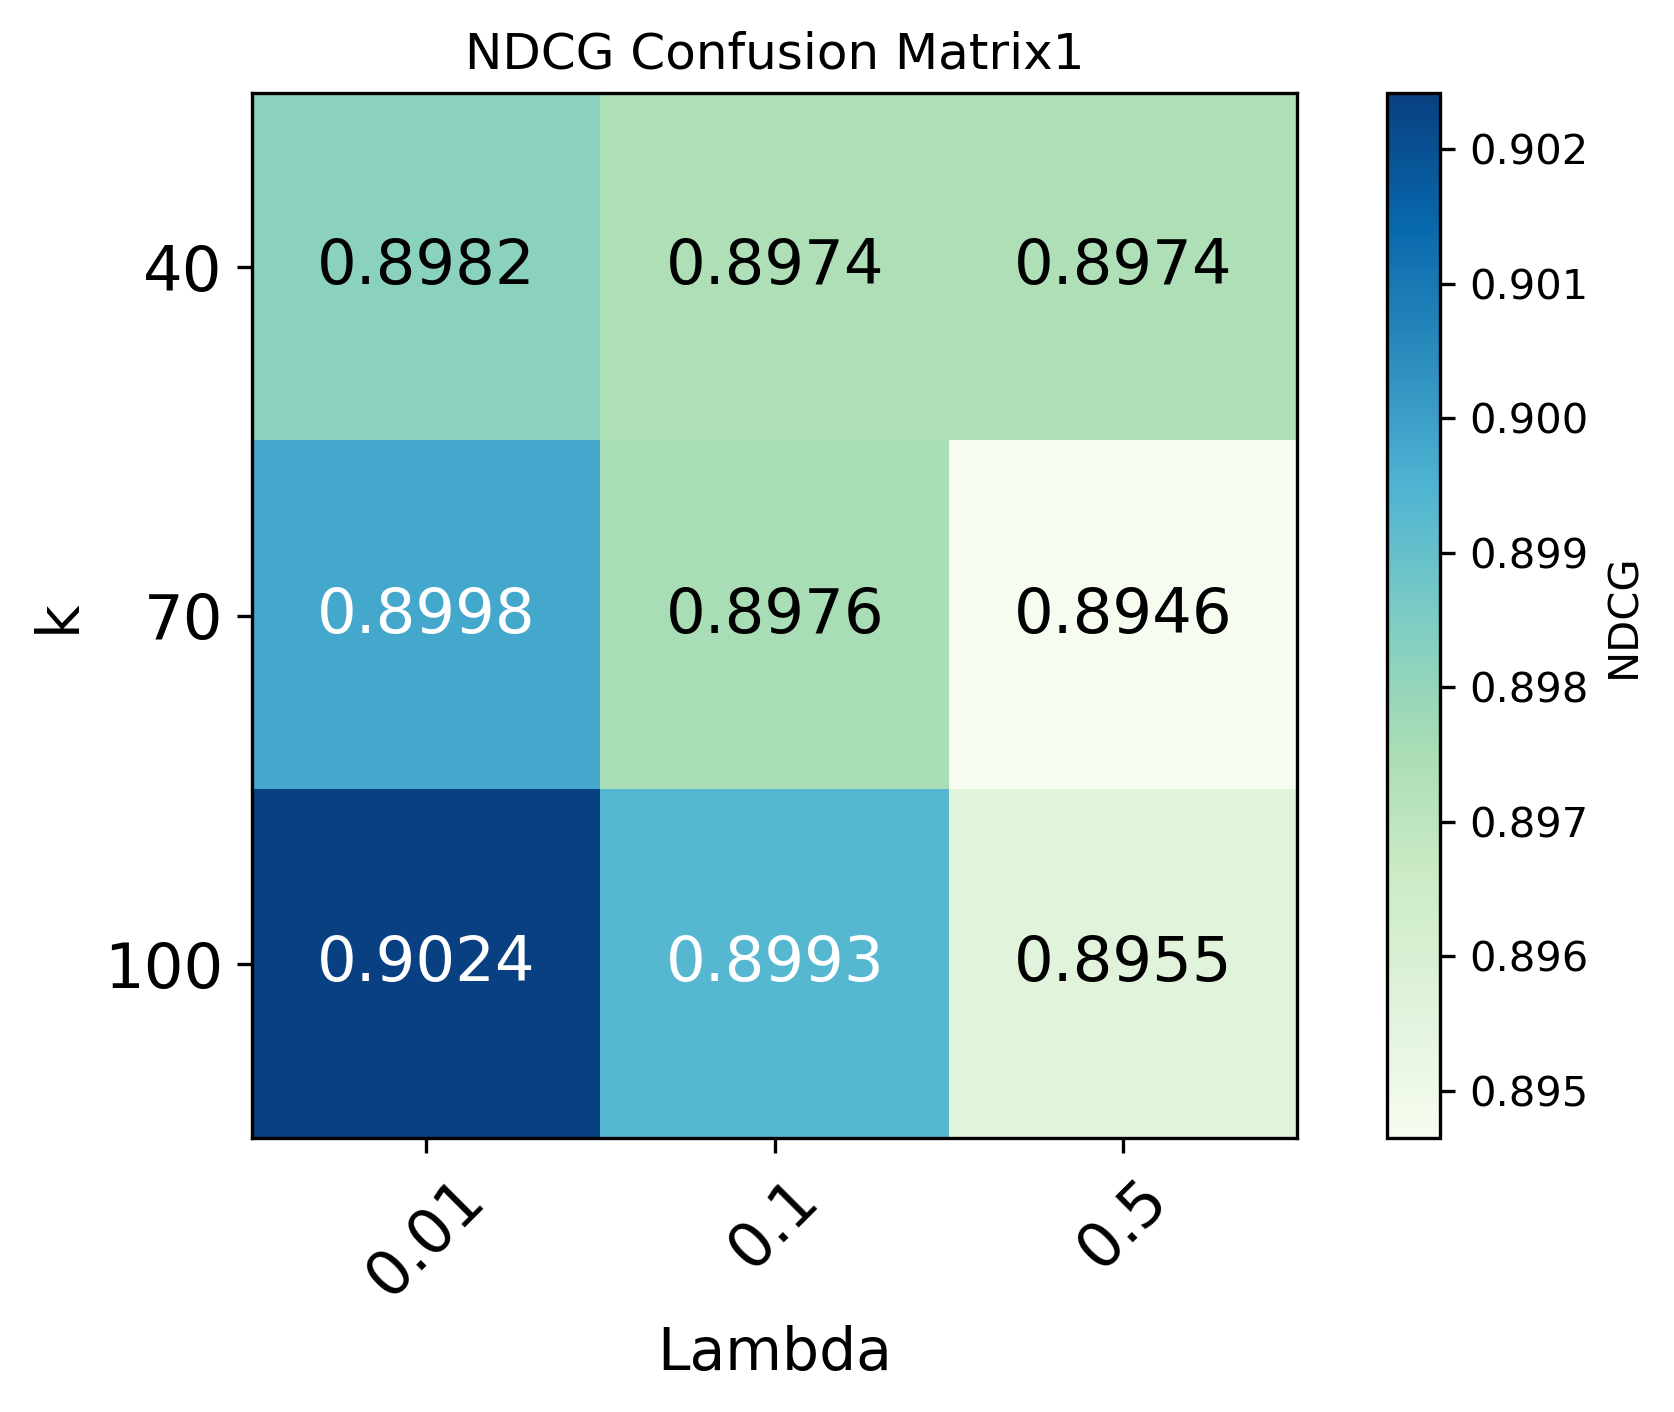
\includegraphics[width=0.39\linewidth]{Confusion_ndcg_1.png}}
    \quad %默认情况下两个子图之间空的较少,使用这个命令加大宽度
    \subfigure[实验1的NDCG折线图]{
        \label{level.sub.2}
		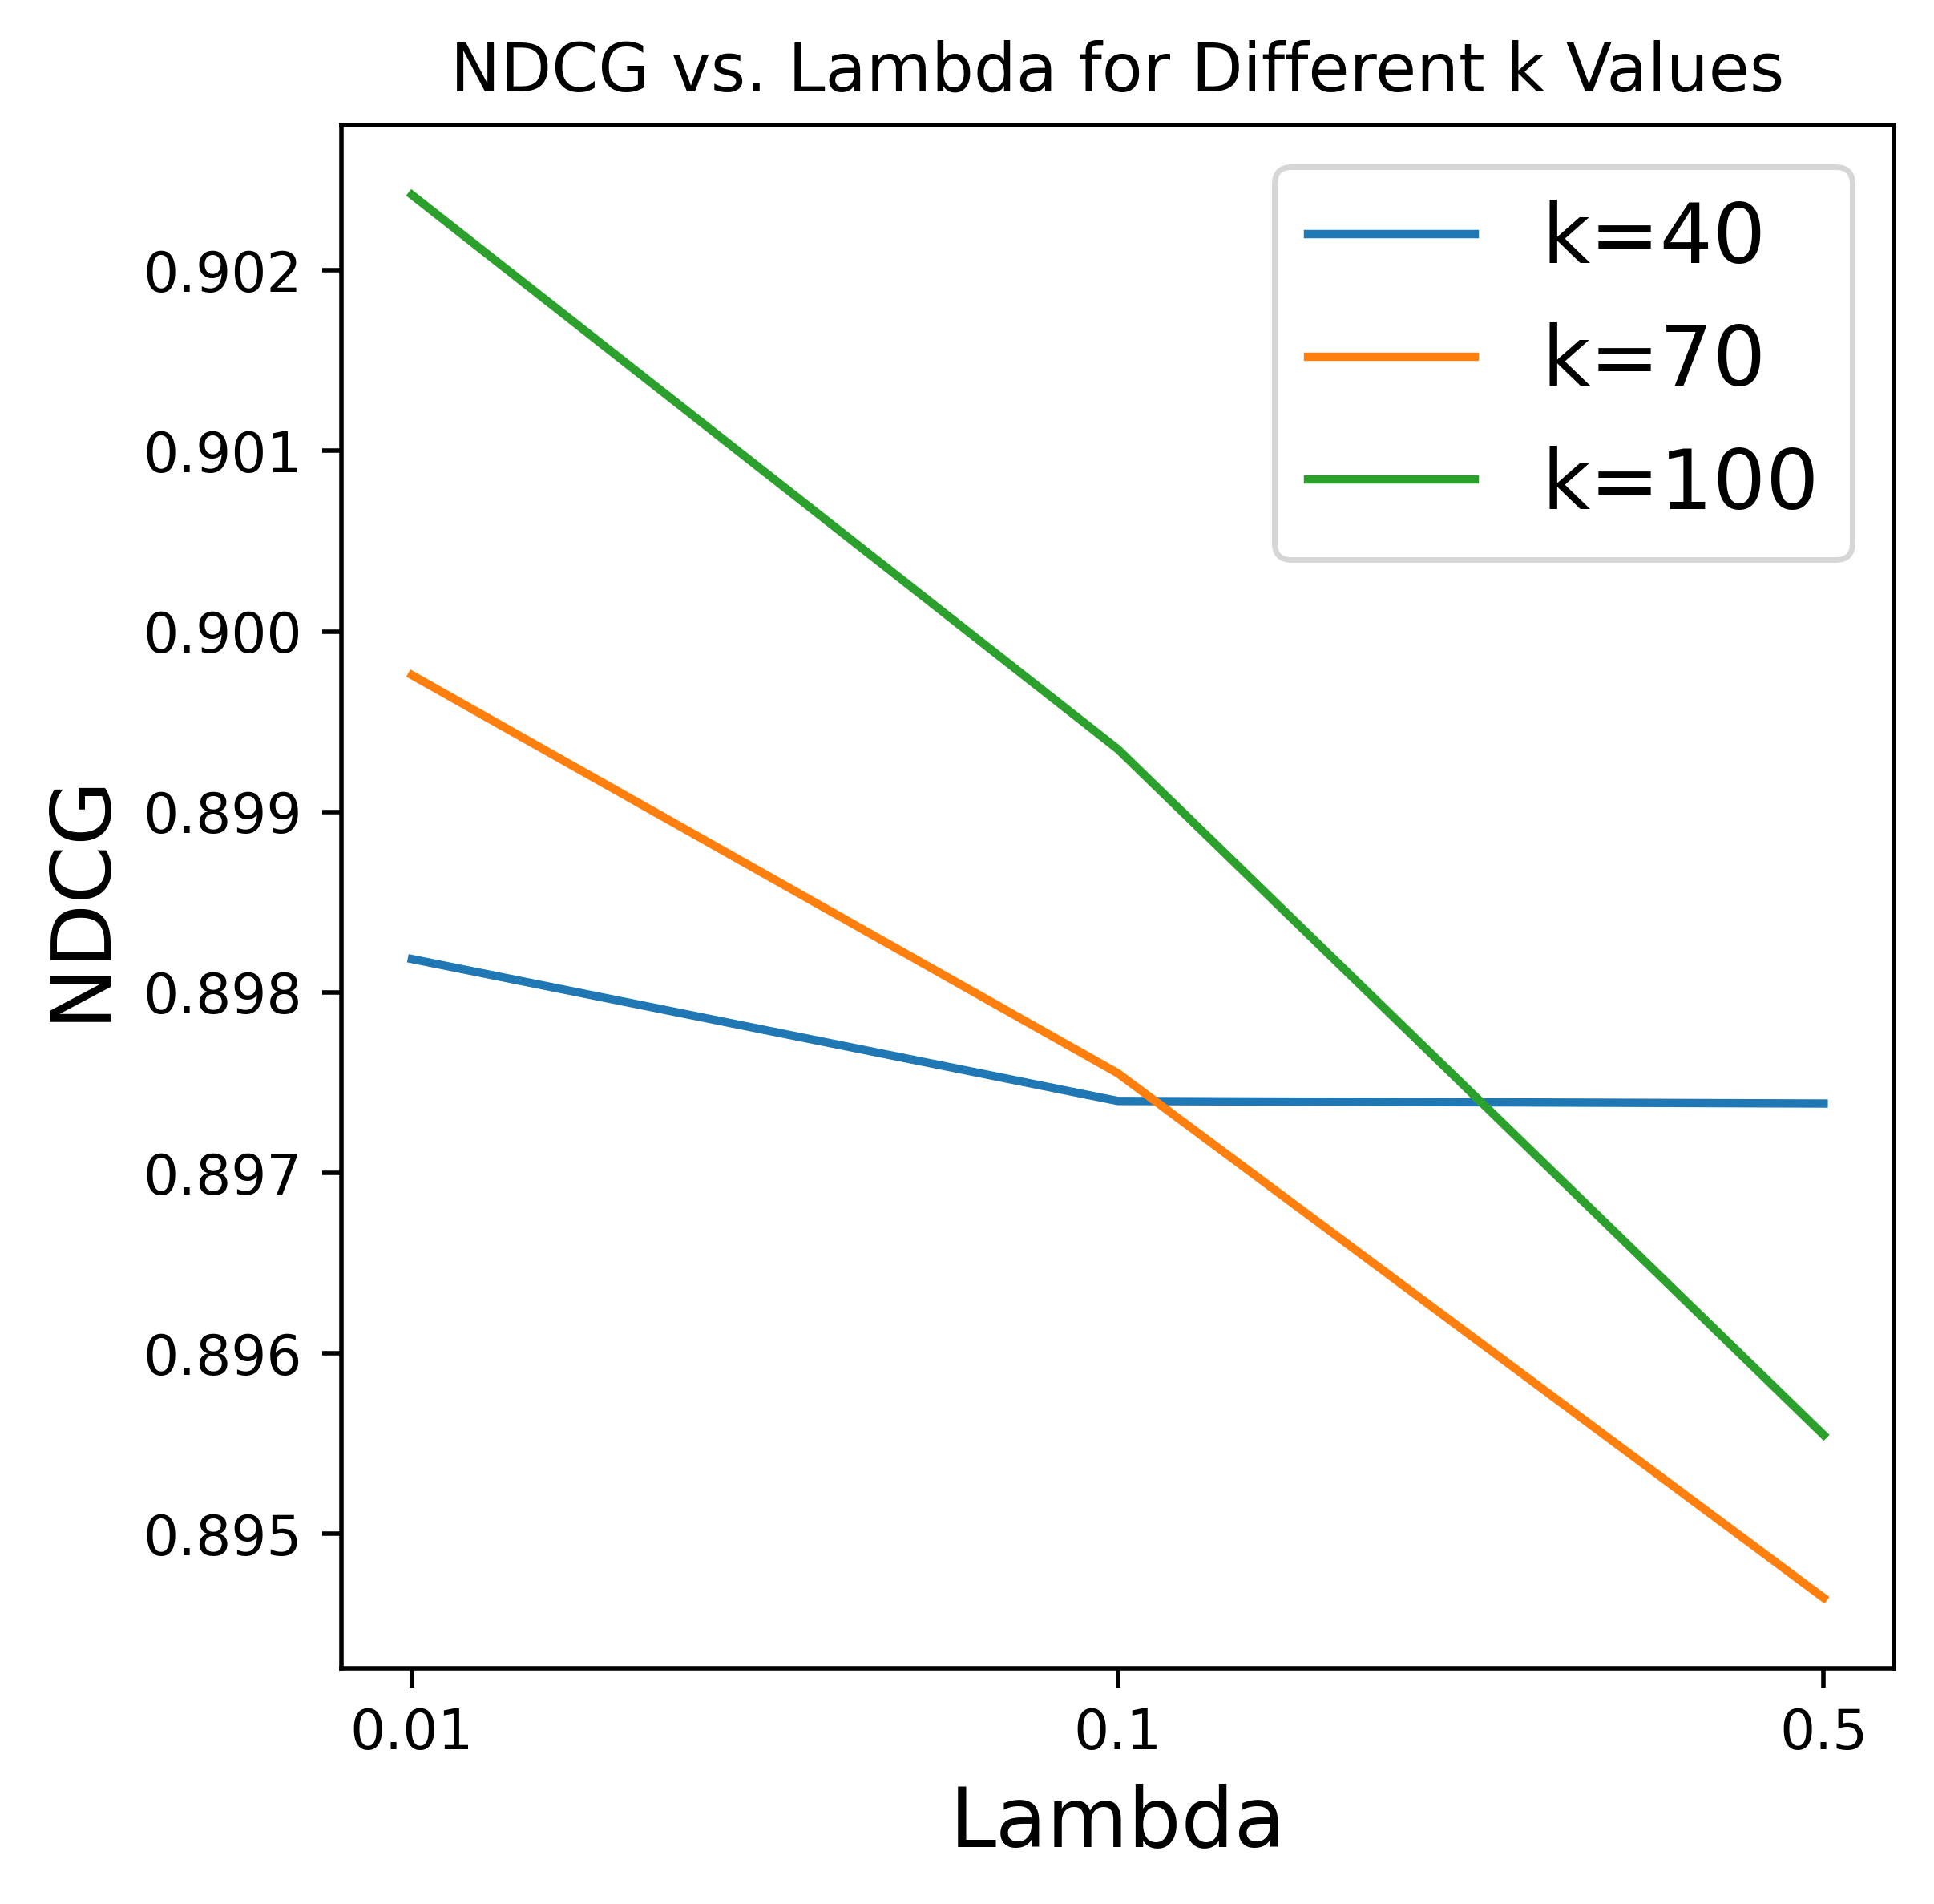
\includegraphics[width=0.33\linewidth]{Lines_ndcg_1.png}}
    %这里是空了一行,能够实现强制将四张图分成两行两列显示,而不是放不下图了再换行,使用\\也行。
   \subfigure[实验1的MSE热力图]{
		\label{level.sub.3}
		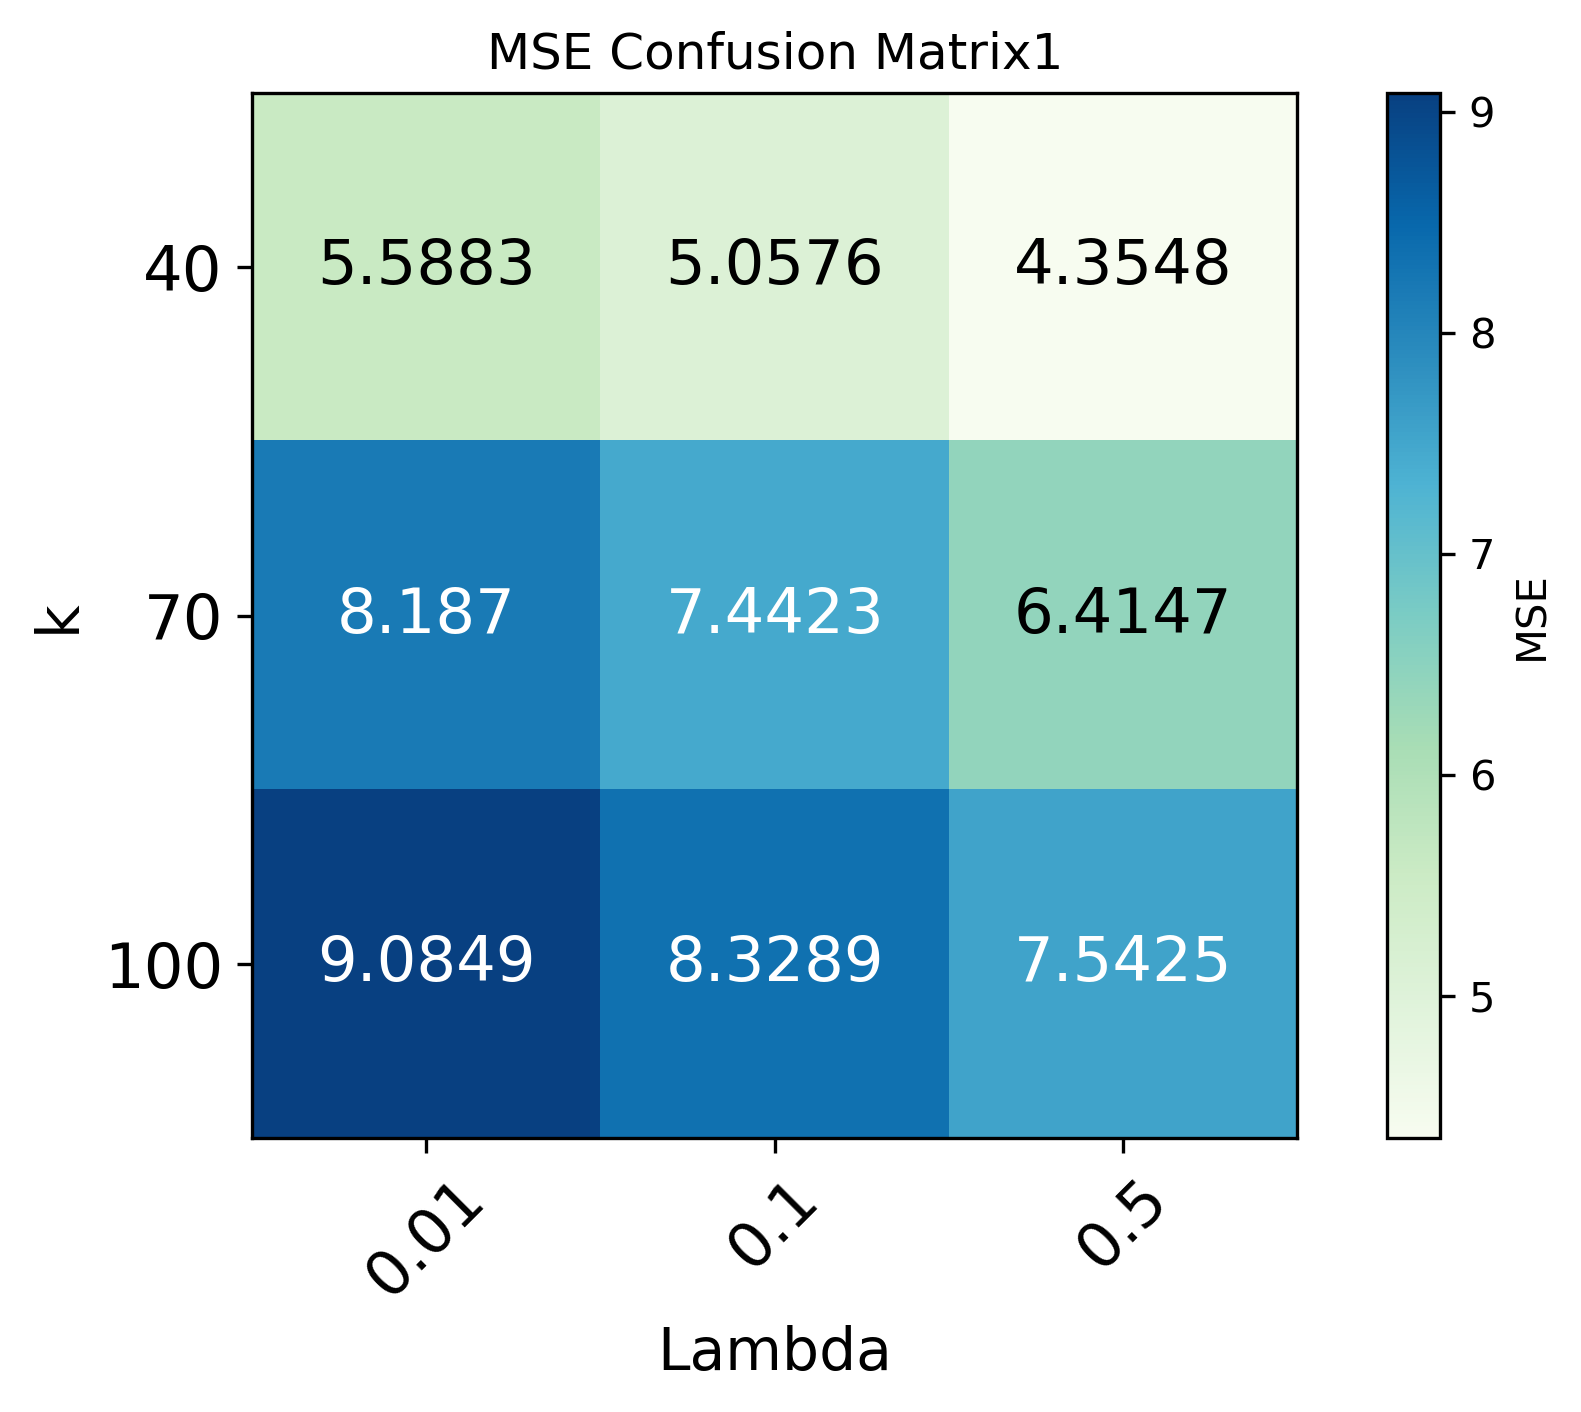
\includegraphics[width=0.38\linewidth]{Confusion_mse_1.png}}
    \quad
    \subfigure[实验1的MSE折线图]{
		\label{level.sub.4}
		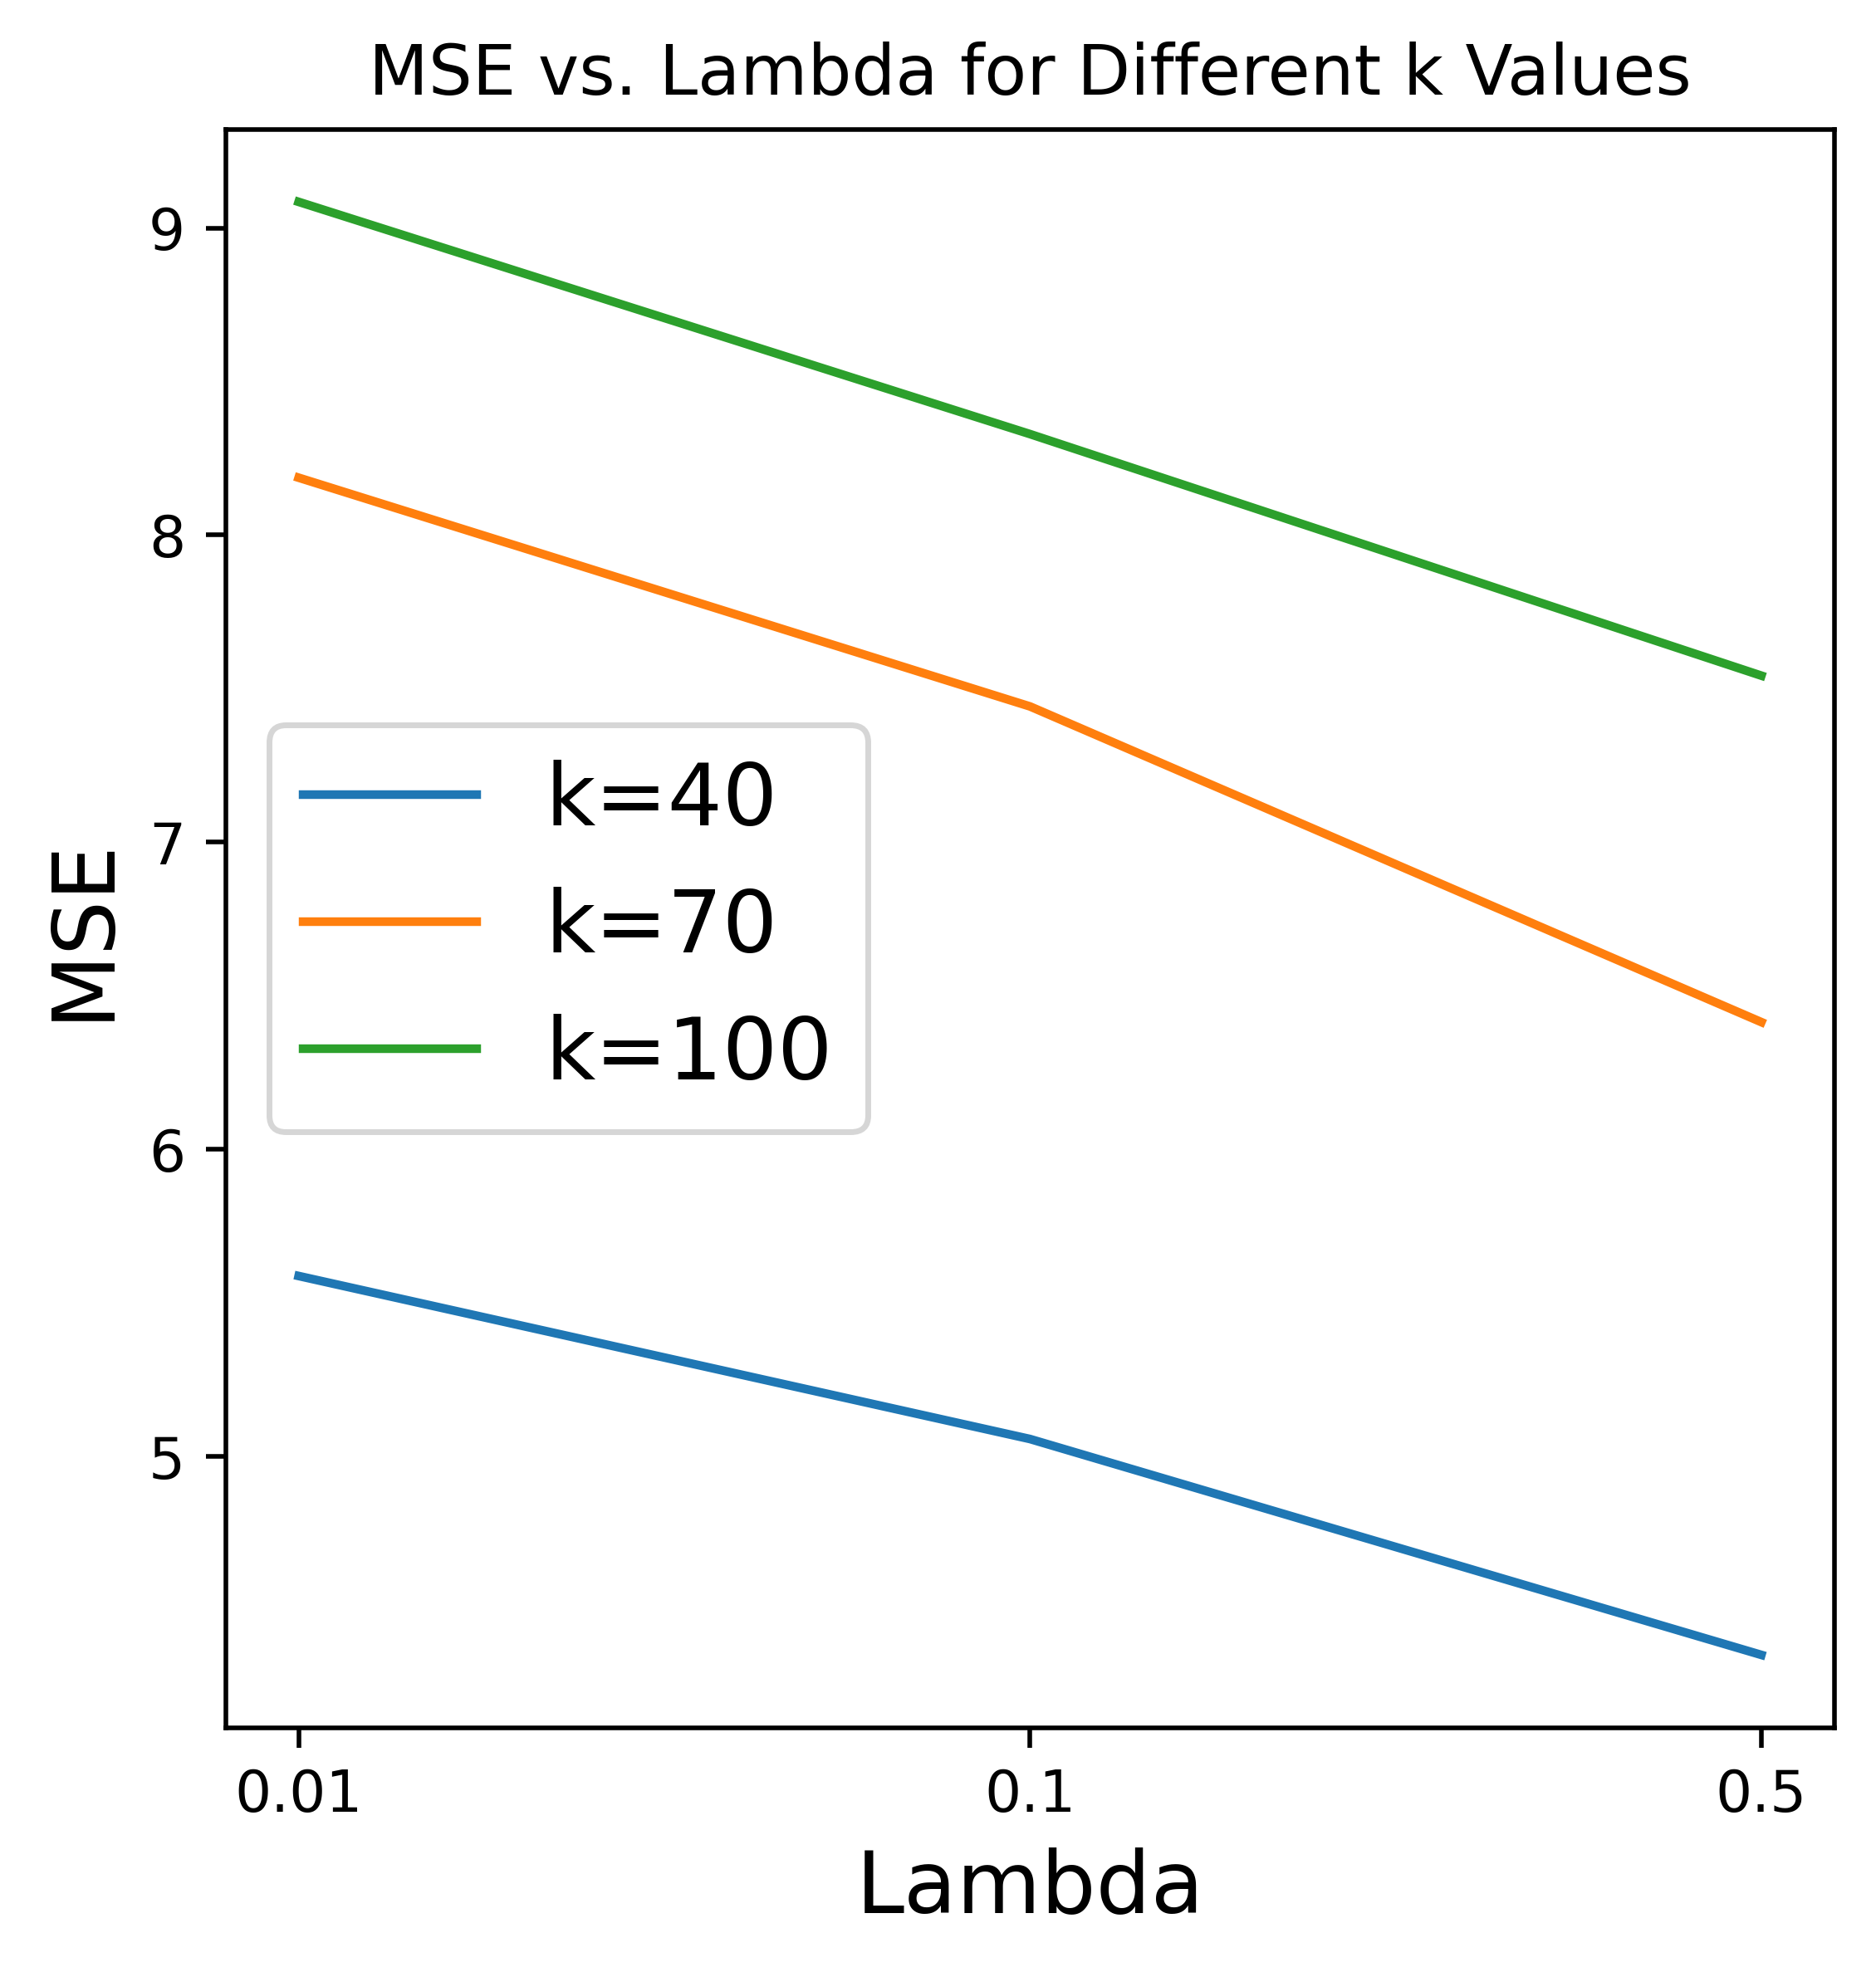
\includegraphics[width=0.31\linewidth]{Lines_mse_1.png}}
    \caption{LFM实验1的效果}
    \label{level}
 \end{figure}

图1中,考虑NDCG指标,总体而言在$k$=100时模型的效果最好,并且对于不同的$k$值而言,都在正则化参数越大时表现越差,因此在k=40,70,100和$\lambda$=0.01,0.1,0.5的量级下,$\lambda$越小明显对模型的提升更大,而且K在100附近更优,NDCG达到了0.90。但是K=100时的计算速度非常慢,并不理想。此外,实验1中NDCG越大(表现越好)和MSE越小(表现越差)竟然同时出现,而理想的最优模型应该同时满足NDCG值大且MSE值小。故实验1并没有找到综合效果最好的模型,需要继续实验。

进一步设计实验2,希望找到速度更快的方法。图2显示$k=20$时的NDCG在0.91以上,明显超过了实验一的最佳模型,在MSE上的表现也远远优于实验1. 并且此时训练模型的时长大大降低,故选定\textbf{隐特征大小k=20,正则化参数$\lambda$=0.1}.


\begin{figure}[H] %这里使用的是强制位置,除非真的放不下,不然就是写在哪里图就放在哪里,不会乱动
    \centering  %图片全局居中
    \vspace{-0.35cm} %设置与上面正文的距离
    \subfigtopskip=2pt %设置子图与上面正文或别的内容的距离
    \subfigbottomskip=2pt %设置第二行子图与第一行子图的距离,即下面的头与上面的脚的距离
    \subfigcapskip=-5pt %设置子图与子标题之间的距离
    \subfigure[实验2的NDCG热力图]{
        \label{level2.sub.1}
        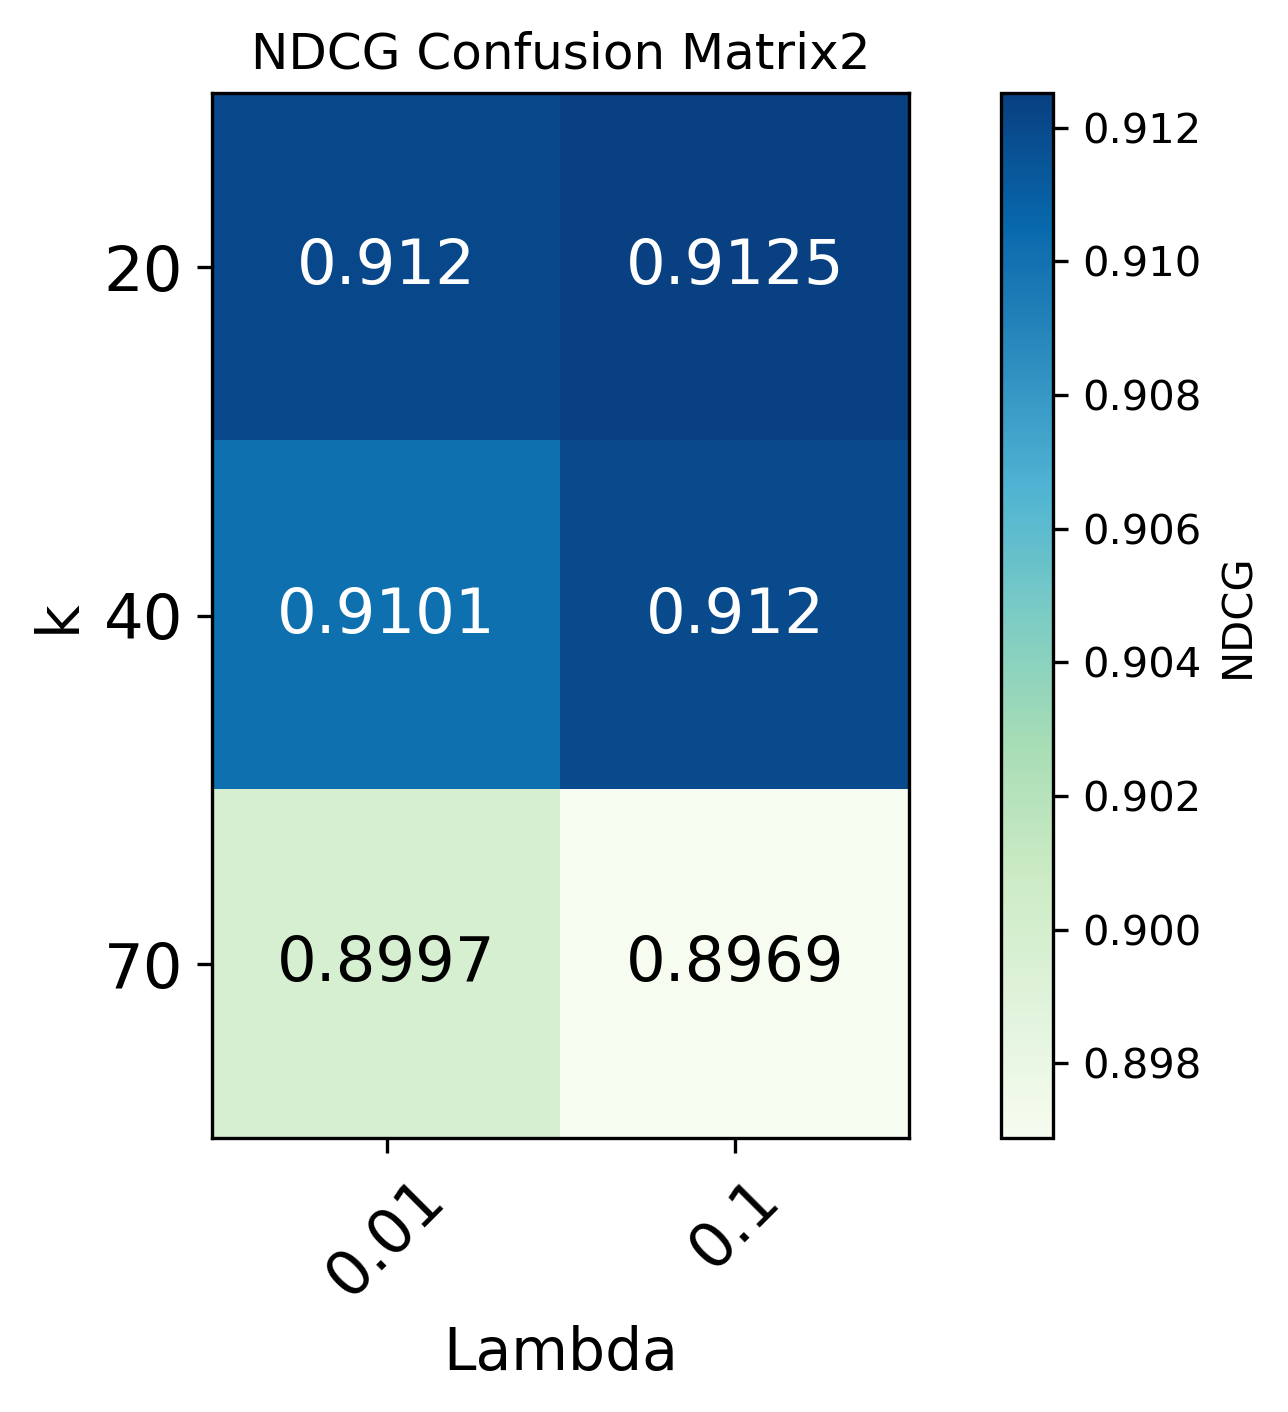
\includegraphics[width=0.32\linewidth]{Confusion_ndcg_2.png}}
    \quad %默认情况下两个子图之间空的较少,使用这个命令加大宽度
    \subfigure[实验2的NDCG折线图]{
        \label{level2.sub.2}
		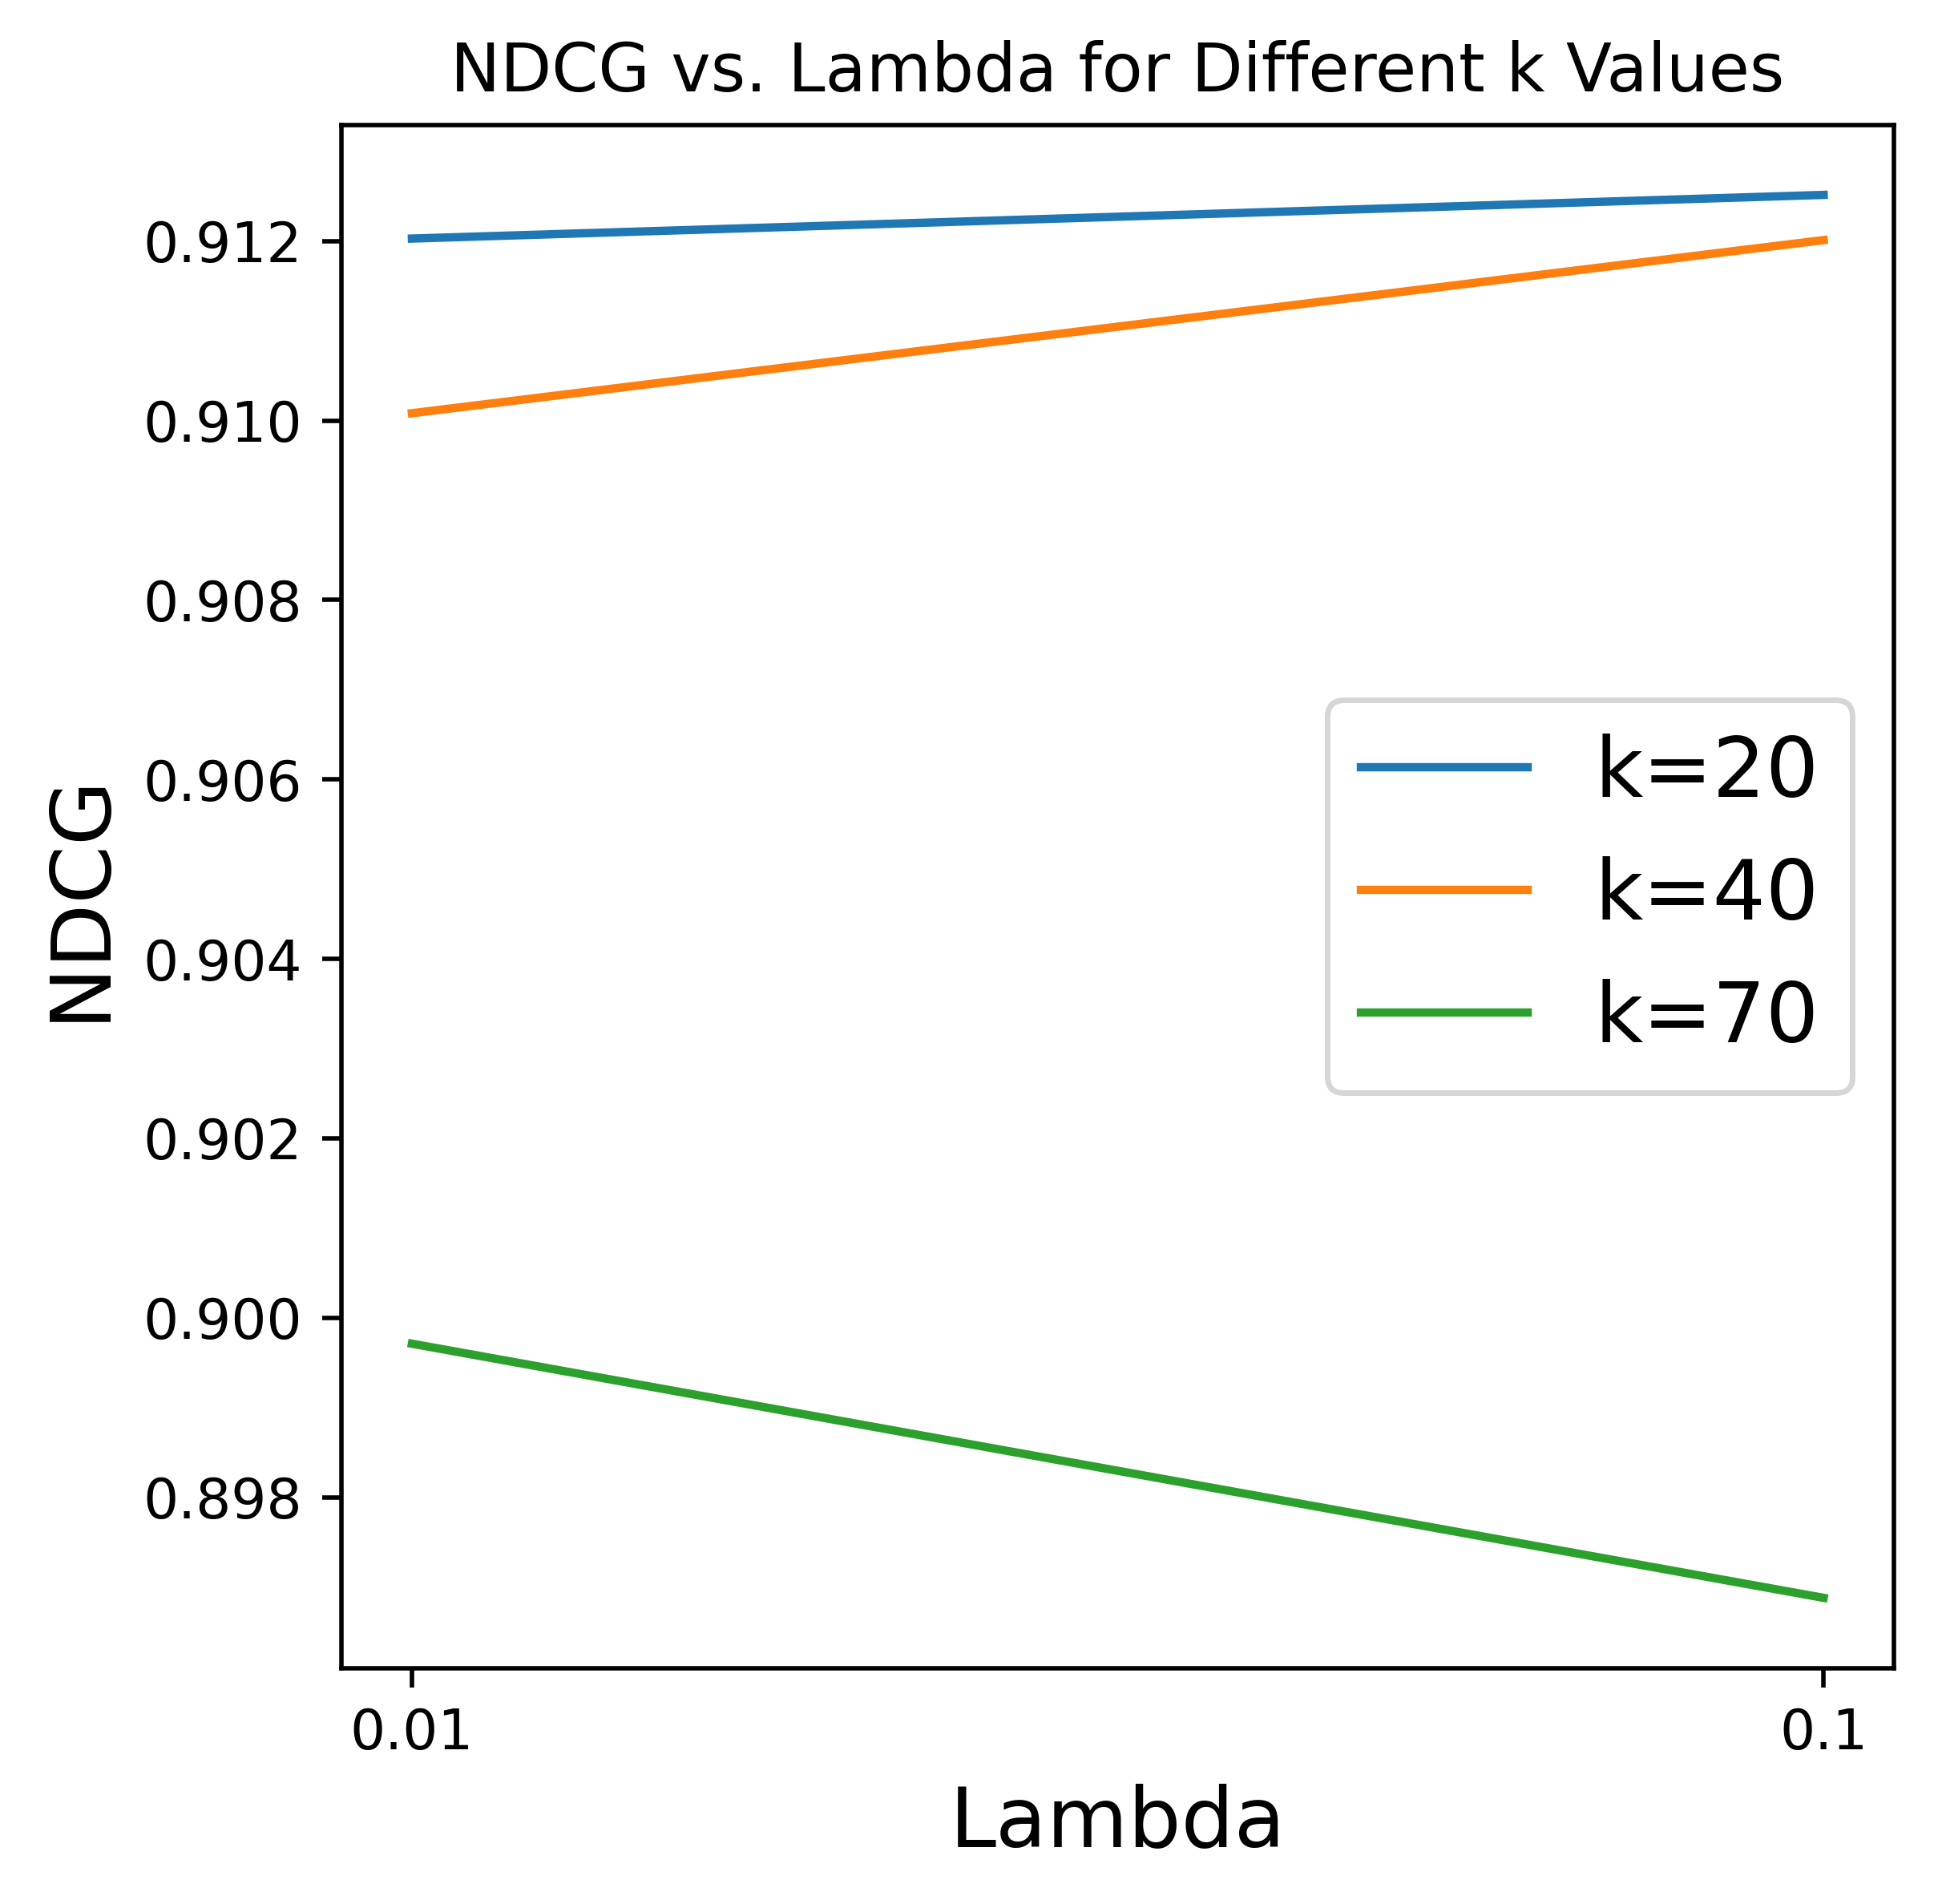
\includegraphics[width=0.33\linewidth]{Lines_ndcg_2.png}}
    %这里是空了一行,能够实现强制将四张图分成两行两列显示,而不是放不下图了再换行,使用\\也行。
   \subfigure[实验2的MSE热力图]{
		\label{level2.sub.3}
		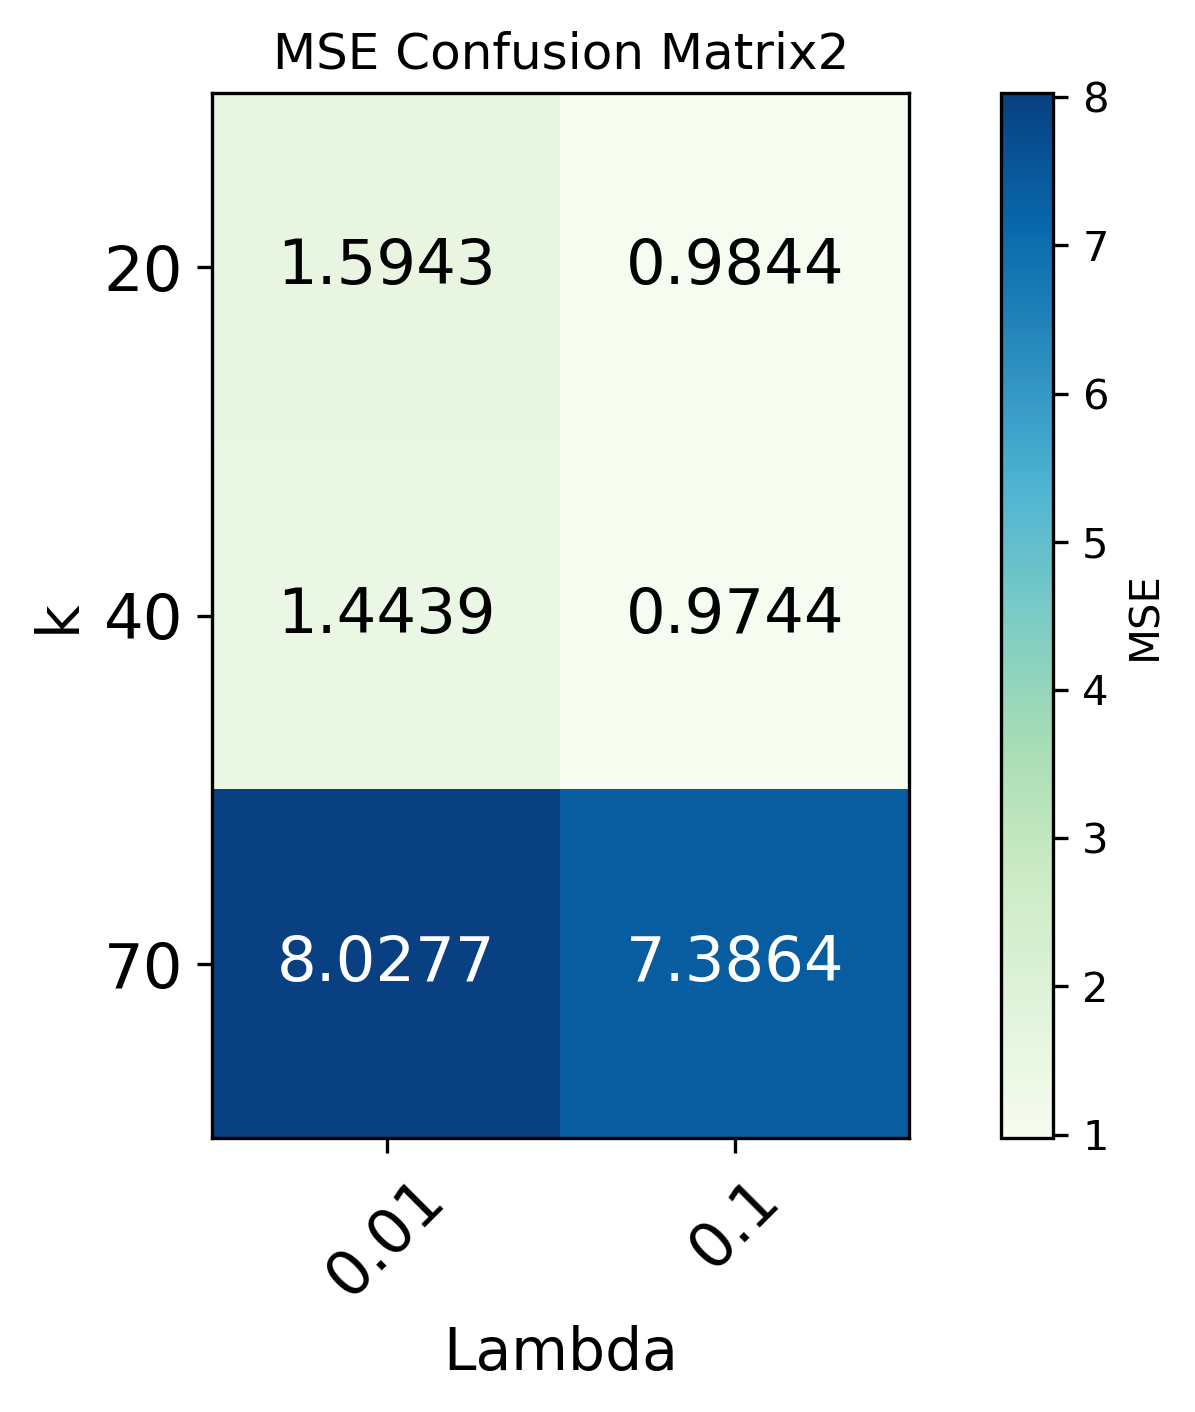
\includegraphics[width=0.30\linewidth]{Confusion_mse_2.png}}
    \quad
    \subfigure[实验2的MSE折线图]{
		\label{level2.sub.4}
		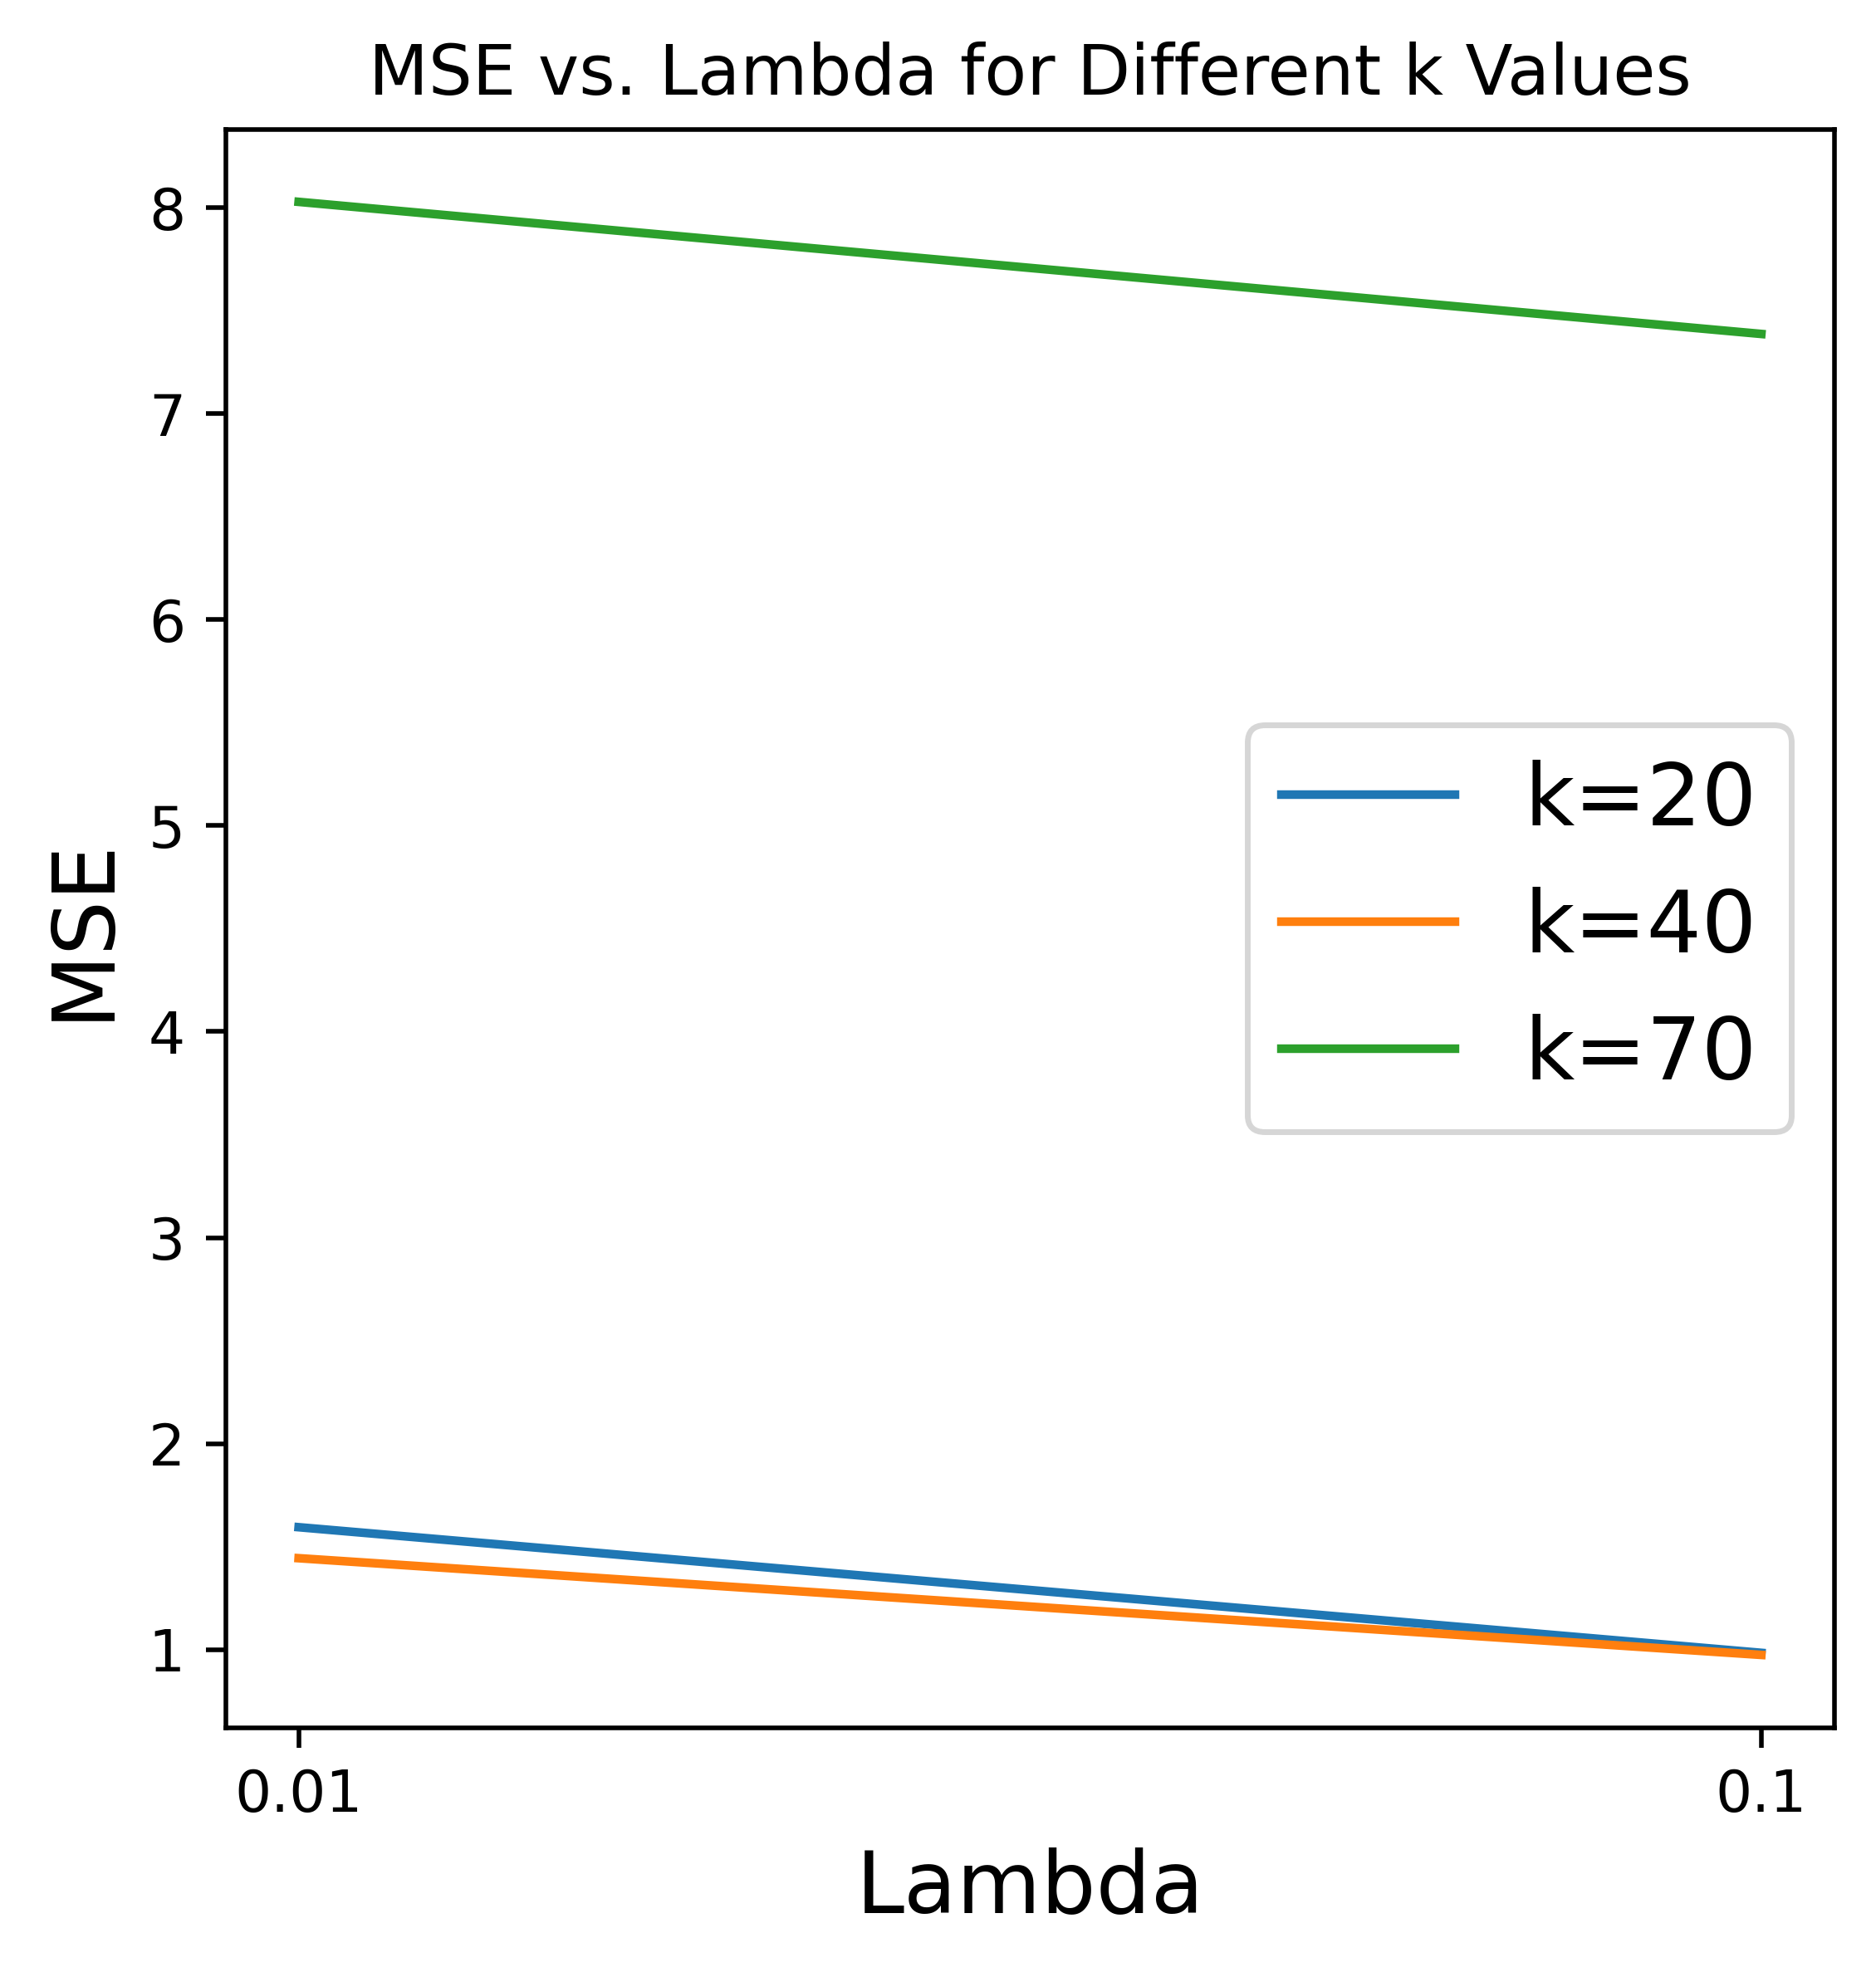
\includegraphics[width=0.31\linewidth]{Lines_mse_2.png}}
    \caption{LFM实验2的效果}
    \label{level2}
 \end{figure}



\subsection{预测结果}

使用\textbf{隐特征大小k=20,正则化参数$\lambda$=0.1,学习率$\alpha=0.01$,最大迭代次数$n=200$,收敛边界$\epsilon=0.001$}的LFM模型,模型表现如下:
\begin{itemize}
    \item 训练数据中20\%划分为验证集时,验证集上$\hat{\rm{NDCG}}$ = 0.916,本地模型训练时间为11.55m.
    \item 使用完整训练数据进行训练,在Kaggle平台测试集上$\rm{NDCG}$ = 0.9548(Kaggle id:NaCloudy),本地模型训练时间为11.55m.
\end{itemize}

此外,对于BPR模型,训练需要更长时间(50个epoch需要20分钟,而200次梯度下降需要接近一个小时),因此不对参数进行grid选择。将\textbf{隐特征大小k=20,正则化参数$\lambda$=0.1}的BPR模型提交到kaggle平台,NDCG只有0.9249,远低于LFM模型。

还可以将model-based CF与memory-based CF进行比较。略去参数选择部分,将近邻集合大小为50、相似度阈值为0.1的UCF模型提交在kaggle平台,NDCG值和LFM模型一致。对比而言,UCF模型需要的训练时间短,测试时间为4分钟;而LFM模型的训练时间为接近12分钟。因此对于数据量大、需要频繁推荐、不需要频繁更新系统的情况而言,LFM模型更合适。

\section{提交文件列表}

压缩包\verb|`宋朝芸_10215001419_1`|包含以下这些内容:

\begin{lstlisting}
project_report.pdf

prediction_results
     output_svd_20_0.1_0.001.csv

source_code
     Confusion_grad_1.png  # 第1次实验的在验证集上的gradient热力图
     Confusion_grad_2.png  # 第2次实验的在验证集上的gradient热力图
     Confusion_mse_1.png   # 第1次实验的在验证集上的mse热力图
     Confusion_mse_1.png   # 第1次实验的在验证集上的mse热力图
     Confusion_ndcg_1.png  # 第1次实验的在验证集上的ndcg热力图
     Confusion_ndcg_2.png  # 第2次实验的在验证集上的ndcg热力图
     exp1_grad.csv         # 第1次实验的grad矩阵
     exp1_mse.csv          # 第1次实验的mse矩阵
     exp1_ndcg.csv         # 第1次实验的ndcg矩阵
     exp2_grad.csv         # 第2次实验的grad矩阵
     exp2_mse.csv          # 第2次实验的mse矩阵
     exp2_ndcg.csv         # 第2次实验的ndcg矩阵
     Lines_grad_1.png      # 第1次实验的在验证集上的gradient折线图
     Lines_grad_2.png      # 第2次实验的在验证集上的gradient折线图
     Lines_mse_1.png       # 第1次实验的在验证集上的mse折线图
     Lines_mse_1.png       # 第1次实验的在验证集上的mse折线图
     Lines_ndcg_1.png      # 第1次实验的在验证集上的ndcg折线图
     Lines_ndcg_2.png      # 第2次实验的在验证集上的ndcg折线图
     output_svd_20_0.1_0.001.csv     # 测试集上预测结果
     source_code.ipynb       # 源代码,jupyter notebook形式
     test.csv                # 训练数据文件
     train.csv               # 测试数据文件
     train_.csv              # 修改后的测试数据文件
\end{lstlisting}




\newpage



\end{document}
